
%----------------------------------------------------------------------------------------
%	PACKAGES AND OTHER DOCUMENT CONFIGURATIONS
%----------------------------------------------------------------------------------------

\documentclass[12pt]{article}

\usepackage{graphicx}
\usepackage{epsfig}
\usepackage{psfrag}
%\usepackage{subfigure}
%\usepackage{subfig}
%\usepackage{tabularx}
\usepackage{subfigmat}
\usepackage{subeqnarray}
\usepackage[colorlinks]{hyperref}
\usepackage{amsmath,amsfonts,amsfonts,amsthm}
\usepackage{xcolor,colortbl}
\usepackage[mathscr]{euscript}
\usepackage{algorithm2e}
\usepackage{siunitx}
\usepackage{rotating}
\usepackage{bm}
\setcounter{secnumdepth}{3}
\usepackage[version=3]{mhchem} 
\usepackage{graphicx}
\usepackage{fancyvrb}
\usepackage[top=1in, bottom=1in, left=1in, right=1in]{geometry}
\graphicspath{{../Figures/}}
\usepackage{color}
\usepackage{pdfpages}
\usepackage{enumitem}
\usepackage{bbm}

\newcommand\alignedbox[2]{
	% Argument #1 = before & if there were no box (lhs)
	% Argument #2 = after & if there were no box (rhs)
	&  % Alignment sign of the line
	{
		\settowidth\dlf{$\displaystyle #1$}  
		% The width of \dlf is the width of the lhs, with a displaystyle font
		\addtolength\dlf{\fboxsep+\fboxrule}  
		% Add to it the distance to the box, and the width of the line of the box
		\hspace{-\dlf}  
		% Move everything dlf units to the left, so that & #1 #2 is aligned under #1 & #2
		\boxed{#1 #2}
		% Put a box around lhs and rhs
	}
}
%----------------------------------------------------------------------------------------
%	ABBREVIATIONS SECTIONS
%----------------------------------------------------------------------------------------
 \newcommand{\dod}{\mathrm{C}_{12}\mathrm{H}_{26}}
 \newcommand{\nit}{\mathrm{N}_{2}}
 \newcommand{\ox}{\mathrm{O}_{2}}
 \newcommand{\wat}{\mathrm{H}_{2}\mathrm{O}}
 \newcommand{\cardiox}{\mathrm{C}\mathrm{O}_{2}}

\begin{document}
%
%%%%%%%%%%%%%%%%%%%%%%%%%%%%%%%%%%%%%%%%%%%%%%%%%%%%%%%%%%%%%%%%%%%%%%
%
\makeatletter
\newcommand\rlarrows{\mathop{\operator@font \rightleftarrows}\nolimits}
\makeatother
%
%%%%%%%%%%%%%%%%%%%%%%%%%%%%%%%%%%%%%%%%%%%%%%%%%%%%%%%%%%%%%%%%%%%%%%
\newenvironment{itemizePacked}{
\begin{itemize}
  \setlength{\itemsep}{1pt}
  \setlength{\parskip}{0pt}
  \setlength{\parsep}{0pt}
}{\end{itemize}}
\newenvironment{enumeratePacked}{
\begin{enumerate}
  \setlength{\itemsep}{5pt}
  \setlength{\parskip}{0pt}
  \setlength{\parsep}{0pt}
}{\end{enumerate}}
% abbreviations %%%%%%%%%%%%%%%%%%%%%%%%%%%%%%%%%%%%%%%%%%%%%%%%%%%%%%
%
%\def\codefont{scriptsize}
\newcommand{\f}[2]{{\frac{#1}{#2}}}
\newcommand{\wt}[1]{{\widetilde{#1}}}
\newcommand{\wh}[1]{{\widehat{#1}}}
\newcommand{\wc}[1]{{\widecheck{#1}}}
\newcommand{\chem}[1]{\ensuremath{\mathrm{#1}}}
\newcommand{\lrangle}[1]{{\langle{#1}\rangle}}
\newcommand{\lrcurl}[1]{{\{{#1}\}}}
\newcommand{\ol}[1]{{\overline{#1}}}
%\newcommand{\ul}[1]{{\underline{#1}}}
\newcommand{\tr}{{\scriptscriptstyle\mathsf T}}
\newcommand{\dd}{{\scriptscriptstyle\Delta}}
\newcommand{\eps}{{\varepsilon}}

\def\RPP{reaction progress parameter}

% boldface-italic font
\newcommand{\bfit}[1]{\textbf{\textit{#1}}}

%
% SOME COLORS %%%%%%%%%%%%%%%%%%%%%%%%%%%%%%%%%%%%%%%%%%%%%%%%%%%%%%%%
%
\newcommand{\colred}[1]{{\color{red} #1}}
\newcommand{\colblue}[1]{{\color{blue} #1}}
\newcommand{\colwhite}[1]{{\color{white} #1}}
\newcommand{\colgreen}[1]{{\color{green} #1}}
\newcommand{\colbrown}[1]{{\color{Brown} #1}}
\newcommand{\colfucsia}[1]{{\color{Fuchsia} #1}}
\newcommand{\colBlue}[1]{{\color{Blue} #1}}
\newcommand{\corrections}[1]{{\color{blue}#1}}
\newcommand{\comment}[1]{{\color{blue}\bf{[#1]}}}
%
% FOR COMBUSTION TEXT %%%%%%%%%%%%%%%%%%%%%%%%%%%%%%%%%%%%%%%%%%%%%%%%
%
\def\chist{\chi_{Z,\up{st}}}
\def\chiq{\chi_{Z,\up{q}}}
\def\chii{\chi_{Z,\up{i}}}
%
% Standard TEX-abbreviations used %%%%%%%%%%%%%%%%%%%%%%%%%%%%%%%%%%%%
%
\def\cldbpage{\clearpage{\pagestyle{empty}\cleardoublepage}}
%
% CALIGRAPHICAL SYMBOLS %%%%%%%%%%%%%%%%%%%%%%%%%%%%%%%%%%%%%%%%%%%%%%
%
\def\cA{{\cal{A}}}
\def\cB{{\cal{B}}}
\def\cC{{\cal{C}}}
\def\cO{{\cal{O}}}
\def\cD{{\cal{D}}}
\def\cE{{\cal{E}}}
\def\cF{{\cal{F}}}
\def\cH{{\cal{H}}}
\def\cJ{{\cal{J}}}
\def\cG{{\cal{G}}}
\def\cN{{\cal{N}}}
\def\cL{{\cal{L}}}
\def\cS{{\cal{S}}}
\def\cT{{\cal{T}}}
\def\cU{{\cal{U}}}
\def\cC{{\cal{C}}} 
\def\cZ{{\cal{Z}}}
\def\cM{{\cal{M}}}
\def\cP{{\cal{P}}}
\def\cR{{\cal{R}}}
\def\cV{{\cal{V}}}
\def\cQ{{\cal{Q}}}
%
% NEW FUNCTION NAMES %%%%%%%%%%%%%%%%%%%%%%%%%%%%%%%%%%%%%%%%%%%%%%%%%
%
\def\erf{{\rm{erf}}}
%
% TEXT FONT DEFINITIONS %%%%%%%%%%%%%%%%%%%%%%%%%%%%%%%%%%%%%%%%%%%%%%
%
\def\up{\textup}
\def\p{\partial}
\def\d{\textup d}
\def\D{\displaystyle}
%\def\S{\scriptsize}
\def\OmFint{\iiint\limits_{\OmF}}
\def\OmF{{\Omega_{\cal F}}}
\def\OmA{{\Omega_{\cal A}}}
\def\e{\textup{e}}
\def\i{\textup{i}}
\def\REFUP{\rm{ref}}
\def\REF{_{\REFUP}}
%
% DIMENSIONLESS QUANTITIES %%%%%%%%%%%%%%%%%%%%%%%%%%%%%%%%%%%%%%%%%%%
%
%\def\Re{{\rm{Re}}}
\def\Fr{{\rm{Fr}}}
\def\M{{\rm{M}}}
\def\Ce{{\rm{Ce}}}
\def\Re{{\rm{Re}}}
\def\Rd{{\rm{Rd}}}
\def\Le{{\rm{Le}}}
\def\Da{{\rm{Da}}}
\def\Ka{{\rm{Ka}}}
\def\Nu{{\rm{Nu}}}
\def\Sc{{\rm{Sc}}}
\def\Ri{{\rm{Ri}}}
\def\Ec{{\rm{Ec}}}
\def\Tu{{\rm{Tu}}}
\def\St{{\rm{St}}}
\def\Mi{{\rm{Mi}}}
\def\Ra{{\rm{Ra}}}
\def\Ze{{\rm{Ze}}}
%
% FOR LATEX %%%%%%%%%%%%%%%%%%%%%%%%%%%%%%%%%%%%%%%%%%%%%%%%%%%%%%%%%%
%
 \def\avec{{\mbox{\boldmath$a$}}}
 \def\bvec{{\mbox{\boldmath$b$}}}
 \def\Bvec{{\mbox{\boldmath$B$}}}
 \def\cvec{{\mbox{\boldmath$c$}}}
 \def\dvec{{\mbox{\boldmath$d$}}}
 \def\evec{{\mbox{\boldmath$e$}}}
 \def\Fvec{{\mbox{\boldmath$F$}}}
 \def\Nvec{{\mbox{\boldmath$N$}}}
 \def\fvec{{\mbox{\boldmath$f$}}}
 \def\gvec{{\mbox{\boldmath$g$}}}
 \def\hvec{{\mbox{\boldmath$h$}}}
 \def\ivec{{\mbox{\boldmath$i$}}}
 \def\jvec{{\mbox{\boldmath$j$}}}
 \def\kvec{{\mbox{\boldmath$k$}}}
 \def\pvec{{\mbox{\boldmath$p$}}}
 \def\Pvec{{\mbox{\boldmath$P$}}}
 \def\uvec{{\mbox{\boldmath$u$}}}
 \def\Uvec{{\mbox{\boldmath$U$}}}
 \def\nvec{{\mbox{\boldmath$n$}}}
 \def\tvec{{\mbox{\boldmath$t$}}}
 \def\Rvec{{\mbox{\boldmath$R$}}}
 \def\rvec{{\mbox{\boldmath$r$}}}
 \def\svec{{\mbox{\boldmath$s$}}}
 \def\Svec{{\mbox{\boldmath$S$}}}
 \def\xvec{{\mbox{\boldmath$x$}}}
 \def\vvec{{\mbox{\boldmath$v$}}}
 \def\wvec{{\mbox{\boldmath$w$}}}
 \def\yvec{{\mbox{\boldmath$y$}}}
 \def\mvec{{\mbox{\boldmath$m$}}}
 \def\Xvec{{\mbox{\boldmath$X$}}}
 \def\qvec{{\mbox{\boldmath$q$}}}
 \def\0vec{{\mbox{\boldmath$0$}}}
 \def\xivec{{\mbox{\boldmath$\xi$}}}
 \def\rhovec{{\mbox{\boldmath$\rho$}}}
 \def\wpvec{{\boldsymbol{\wp}}}
 \def\psivec{{\mbox{\boldmath$\psi$}}}
 \def\epsvec{{\mbox{\boldmath$\epsilon$}}}
 \def\phivec{{\mbox{\boldmath$\phi$}}}
 \def\varphivec{{\mbox{\boldmath$\varphi$}}}
 \def\zetavec{{\mbox{\boldmath$\zeta$}}}
 \def\kappavec{{\mbox{\boldmath$\kappa$}}}
 \def\varkappavec{{\pmb{\varkappa}}}
 \def\etavec{{\mbox{\boldmath$\eta$}}}
 \def\Psivec{{\boldsymbol{\Psi}}}
 \def\Phivec{{\boldsymbol{\Phi}}}
 \def\Wvec{{\boldsymbol{W}}}
 \def\Yvec{{\mbox{\boldmath$Y$}}}
 \def\Vvec{{\mbox{\boldmath$V$}}}
 \def\cLvec{{\boldsymbol{\cal{L}}}}
 \def\cMvec{{\boldsymbol{\cal{M}}}}
 \def\omegavec{{\mbox{\boldmath$\omega$}}}
 \def\Omegavec{{\mbox{\boldmath$\Omega$}}}
 \def\sigmavec{{\boldsymbol{\sigma}}}
 \def\Amat{{\underline{\underline{{A}}}}}
 \def\Bmat{{\underline{\underline{{B}}}}}
 \def\Phimat{{\underline{\underline{{\Phi}}}}}
 \def\taumat{{\underline{\underline{{\tau}}}}}
 \def\sigmamat{{\underline{\underline{{\sigma}}}}}
 \def\Cmat{{\underline{\underline{{C}}}}}
 \def\Imat{{\underline{\underline{{I}}}}}
 \def\Jmat{{\underline{\underline{{J}}}}}
 \def\Smat{{\underline{\underline{{S}}}}}
 \def\Rmat{{\underline{\underline{{R}}}}}
 \def\Tmat{{\underline{\underline{{T}}}}}
 \def\Emat{{\underline{\underline{{E}}}}}
 \def\tmat{{\underline{\underline{{t}}}}}

 \def\alphavec{{\boldsymbol{\alpha}}}
 \def\betavec{{\boldsymbol{\beta}}}
 \def\tauvec{{\boldsymbol{\tau}}}
 \def\thetavec{{\boldsymbol{\theta}}}
 \def\lambdavec{{\mbox{\boldmath$\lambda$}}}
 \def\cTmat{{\underline{\underline{{\cal{T}}}}}}
 \def\cLmat{{\underline{\underline{{\cal{L}}}}}}
 \def\cMmat{{\underline{\underline{{\cal{M}}}}}}
 \def\kappamat{{\underline{\underline{{\kappa}}}}}
%
% Grad, Div, ... %%%%%%%%%%%%%%%%%%%%%%%%%%%%%%%%%%%%%%%%%%%%%%%%%%%%%
%
\def\Grad{\nabla}
\def\Div{\nabla \cdot}
\def\Lap{\nabla^2}
%

\begin{titlepage}

\newcommand{\ddz}[1]{\frac{\mathrm{d} #1}{\mathrm{d} z}}
\newcommand{\HRule}{\rule{\linewidth}{0.5mm}} % Defines a new command for the horizontal lines, change thickness here

\center % Center everything on the page
 

 
%----------------------------------------------------------------------------------------
%	HEADING SECTIONS
%----------------------------------------------------------------------------------------


%\textsc{\Large STANFORD UNIVERSITY}\\[1.5cm] % Name of your university/college

%----------------------------------------------------------------------------------------
%	TITLE SECTION
%----------------------------------------------------------------------------------------

\HRule \\[1 cm]
{ \huge \bfseries Problem Set 3 Solutions}\\[0.4cm] % Title of your document
\HRule \\[2cm]
 
%----------------------------------------------------------------------------------------
%	AUTHOR SECTION
%----------------------------------------------------------------------------------------

\Large  \textsc{Matthias Ihme}\\[2cm] % Your name
\textsc{\large ME 257/357: Propulsion System and Gas-Turbine Analysis}\\[2cm] % Major heading such as course name

%----------------------------------------------------------------------------------------
%	LOGO SECTION
%----------------------------------------------------------------------------------------

\includegraphics[width=50mm]{stanford_seal.png}\\[2cm] % Include a department/university logo - this will require the graphicx package
%----------------------------------------------------------------------------------------
%----------------------------------------------------------------------------------------
%	DATE SECTION
%----------------------------------------------------------------------------------------
{\large Spring 2018}%\\[3cm] % Date, change the \today to a set date if you want to be precise

\vfill % Fill the rest of the page with whitespace

\end{titlepage}

%----------------------------------------------------------------------------------------
%	BODY SECTION
%----------------------------------------------------------------------------------------

%%%%%%%%%%%%%%%%%%%%%%%%%%%%%%%%%%%%%%%%%%%%%%%%%%%%%%%%%%%%%%%%%%%%%%%%%%%%%%%%  
\section{Problem 1: Turbofan with Combustion Model (30 pts)}
	\begin{enumerate}[label=(\alph*)]
		\item (10 pts)
			Example code uploaded to Canvas.
		\item (20 pts)
			\begin{enumerate}[label=(\roman*)]
				\item (10 pts)
					A plot of the real turbofan thrust is shown in Fig.~\ref{FIG_1ptbi}. Thrust is optimized at approximately $\boxed{\phi=1.09,\ 1.05,\ \mathrm{and},\ 1.09}$ for $h=$ 0, 30, and 43 kft, respectively. Thrust is peaking near the stoichiometric condition since an optimal amount of fuel is being consumed for this condition given the mass flow of the air.
					\begin{figure}[!t!]
						\begin{center}
							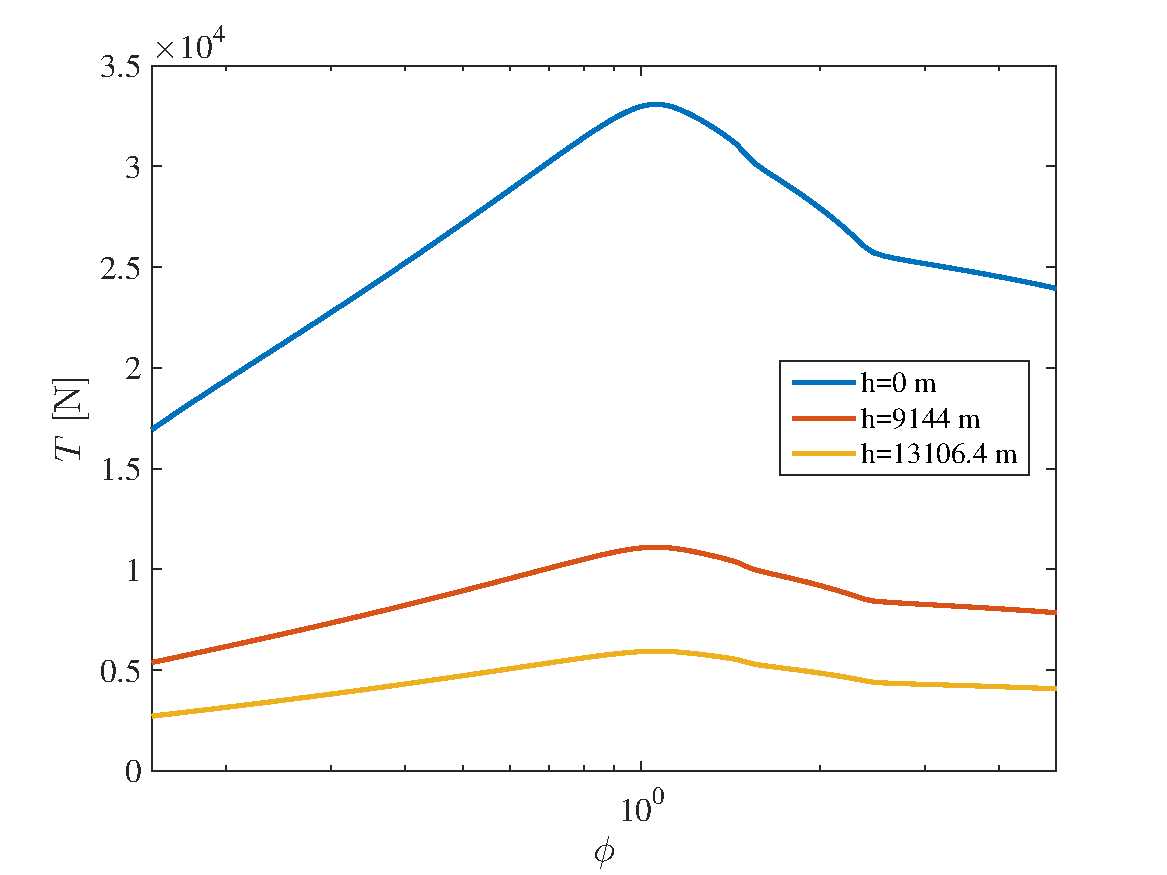
\includegraphics[width=120mm]{problem1ptbi.pdf}
							\caption{\label{FIG_1ptbi} Thrust computed for the equilibrium combustion model.}
						\end{center}
					\end{figure}
				\item (10 pts)
					A plot of the temperature ratio is shown in Fig.~\ref{FIG_1ptbii}. The temperature ratio peaks at approximately $\boxed{\phi=1.09,\ 1.09,\ \mathrm{and},\ 1.05}$ for $h=$ 0, 30, and 43 kft, respectively. $T_4/T_{4,\max}=1$ at approximately $\boxed{\phi=0.34,\ 0.4,\ \mathrm{and},\ 0.4}$ for $h=$ 0, 30, and 43 kft, respectively. Comparing to Fig.~\ref{FIG_1ptbi}, these equivalence ratios are $\boxed{\mathrm{suboptimal}}$.
					\begin{figure}[!t!]
						\begin{center}
							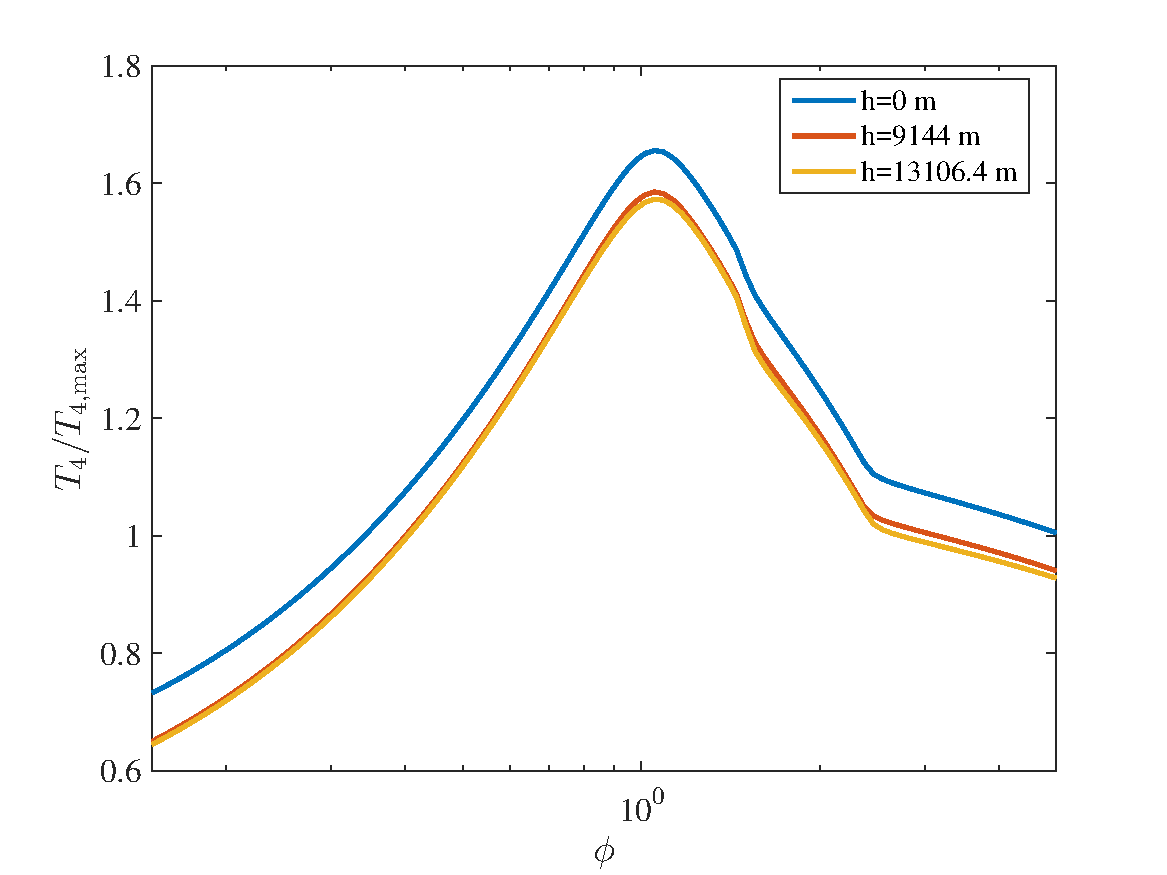
\includegraphics[width=120mm]{problem1ptbii.pdf}
							\caption{\label{FIG_1ptbii} Temperature ratio computed for the equilibrium combustion model.}
						\end{center}
					\end{figure}
			\end{enumerate}
	\end{enumerate}
%%%%%%%%%%%%%%%%%%%%%%%%%%%%%%%%%%%%%%%%%%%%%%%%%%%%%%%%%%%%%%%%%%%%%%%%%%%%%%%%  
\section{Problem 2: Cruise Conditions for the HondaJet (30 pts)}
	\begin{enumerate}[label=(\alph*)]
		\item (5 pts)
			We will use the core airflow, $\dot{m}_c$, and the bypass ratio, $\beta$ in addition to the pressure ratios and the aircraft parameters. However, we will not use  the$T_{04}=1600$ specification. We will compute $T_{04}$ as the adiabatic flame temperature, and will find $\dot{m}_f$ from the more accurate combustor model.
		\item (10 pts)
			Note that the HondaJet has two engines and this must be accounted for. The entire drag is given by
			\begin{equation}
				D=\frac{\rho_0 U_0^2SC_{D,0}}{2}+\frac{2W^2}{\pi e \rho_0 U_0^2 b^2}\ .
			\end{equation}
			Hence the thrust required for one engine is $T^*=D/2$, while the mass flow through each engine is still $\dot{m}_c=\dot{m}_{c,\mathrm{SL}}\rho_0/\rho_{0,\mathrm{SL}}=8\rho_0/\rho_{0,\mathrm{SL}}$ kg/s. Finally, accounting for both engines burning fuel, $\dot{m}_{f,\mathrm{total}}=2\dot{m}_f$
		\item (5 pts)
			The ODE is simply 
			\begin{equation}
				\frac{\d W }{\d t}=-\dot{m}_{f,\mathrm{total}}g\ .
			\end{equation}
			$\dot{m}_{f,\mathrm{total}}$ depends on producing a certain amount of thrust; so, engine parameters as well as drag matters. Also, drag is a function of altitude, airspeed, and aircraft parameters.
		\item (5 pts)
			Using a airspeed of 200 m/s and an altitude of 43 kft, the range is found to be \boxed{6360\ \mathrm{km}}.
		\item (5 pts)
			The Breguet range equation predicts $s_{43\mathrm{kft.}}\in[2810,3590]$, which is significantly less than that given by the more realistic combustor. Differences include the incorporation of a non-constant $L/D$ ratio, and a significantly lower TSFC.
	\end{enumerate}
%%%%%%%%%%%%%%%%%%%%%%%%%%%%%%%%%%%%%%%%%%%%%%%%%%%%%%%%%%%%%%%%%%%%%%%%%%%%%%%%  
\section{Problem 3: Turbofan with Combustion Model (30 pts)}
	\begin{enumerate}[label=(\alph*)]
		\item (10 pts)
			A plot showing the normalized mass flow rate of NO is shown in Fig.~\ref{FIG_3}. An equivalence ratio of $\phi=1.42$ is shown to meet the standard. However at this rich equivalence ratio, carbon monoxide and particulate formation may become an issue.
			\begin{figure}[!t!]
				\begin{center}
					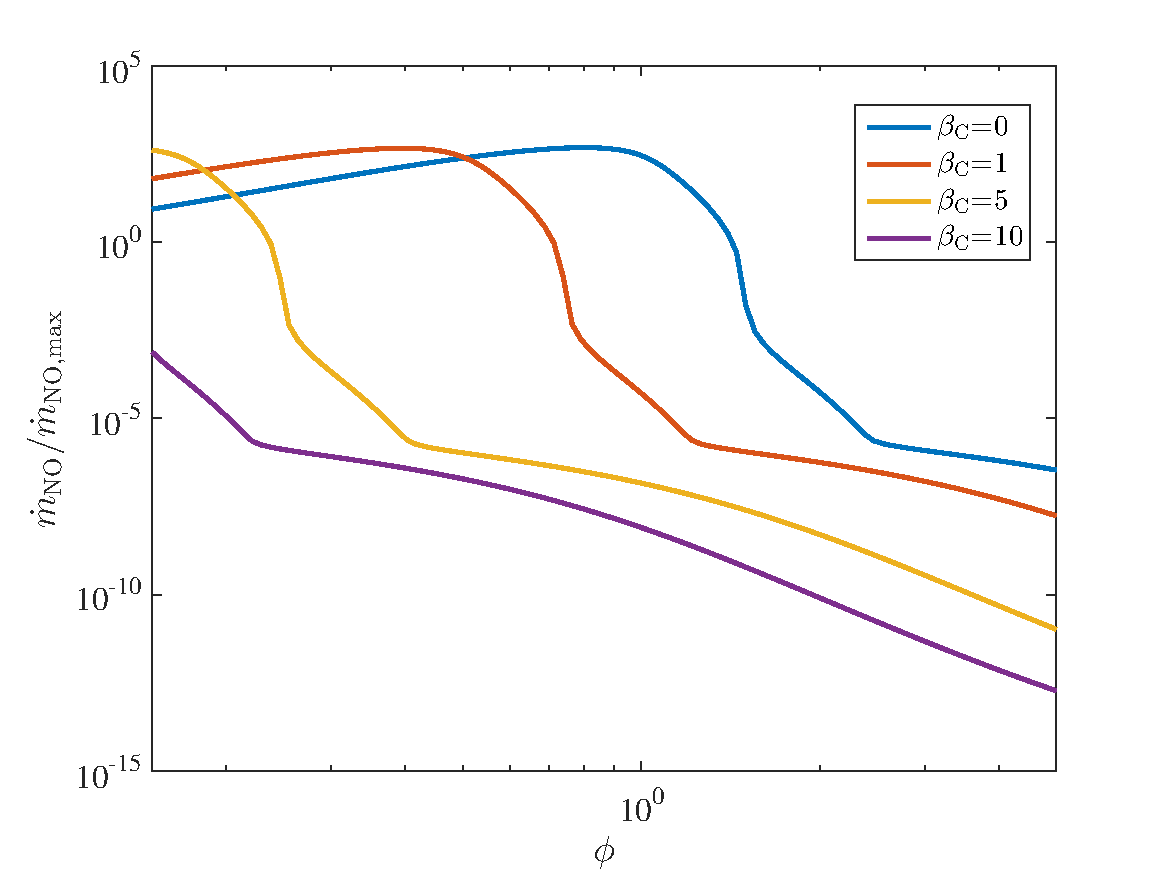
\includegraphics[width=120mm]{problem3.pdf}
					\caption{\label{FIG_3} Mass flow rate of nitric oxide against the combustor reroute ratio.}
				\end{center}
			\end{figure}
		\item (15 pts)
			\begin{enumerate}
				\item (5 pts)
					$L_\mathrm{dil}$ is obtained by
					\begin{equation}
						\begin{aligned}
							\frac{\d \dot{m}_\mathrm{NO}}{\d t}&=k\dot{m}_\mathrm{N_2}\dot{m}_\mathrm{O} \\
							\implies \dot{m}_\mathrm{NO} &= k\dot{m}_\mathrm{N_2}\dot{m}_\mathrm{O}t\\
							 &= k\dot{m}_\mathrm{N_2}\dot{m}_\mathrm{O}\frac{x}{U_4}\\
							 \implies L_\mathrm{dil}&=\boxed{\frac{U_4\dot{m}_\mathrm{NO,\max}}{k\dot{m}_\mathrm{N_2}\dot{m}_\mathrm{O}}}\ .
						\end{aligned}
					\end{equation}
					Substituting the given values, one obtains $\boxed{L_\mathrm{dil}=1.3}$ km. Since the maximum dilution distance is much longer than any practical length for a combustor, it is quite feasible to quench the combustion before any significant NO is formed.
				\item (10 pts)
					Figure~\ref{FIG_3} shows the normalized mass production of NO for three reroute ratios. Using the RQL combustor design. It is shown for a reroute ratio of 5 or 10, that NO formation is not a limiting factor for the design since the NO formation is much less than the allowable for $T_4/T_{4,\max}=1$.
			\end{enumerate}
		\item (5 pts)
			At sea level, $T_4=1600$ K and $p_4=25.7$ bar for the real turbofan. Substituting these values into the given correlation, one obtains $\boxed{x_\mathrm{NO}=0.0019}$.
			
			For n-dodecane $f_\mathrm{st}=0.0669$, and since from Fig.~\ref{FIG_3} $\phi=0.34$ for $h=0$, $f=\phi f_\mathrm{st}=0.023$. Hence, $\dot{m}_4=(1+f)\dot{m}_3=8.2$ kg/s.
			
			Using the combustor model at the prescribed flight speed and altitude, and $\phi=0.34$, one finds by substituting the computed mole fraction of nitric oxide into the cantera gas object that $Y_\mathrm{NO}=0.002$. Since $\dot{m}_\mathrm{NO}=Y_\mathrm{NO}\dot{m}_4$, $\boxed{\dot{m}_\mathrm{NO}=16.2}$ g/s. Since $\dot{m}_\mathrm{NO}>\dot{m}_{\mathrm{NO},\max}$, this correlation shows that the Honda Jet would not meet the standards. The small difference in the models can likely attributed to the error introduced from the curve-fitting procedure and differences in the species included between the two models. 
	\end{enumerate}
			
%%%%%%%%%%%%%%%%%%%%%%%%%%%%%%%%%%%%%%%%%%%%%%%%%%%%%%%%%%%%%%%%%%%%%%%%%%%%%%%%  	
\end{document}